\documentclass{article}

\usepackage{graphicx}
\usepackage{tikz}
\usepackage{tikzsymbols}
\usetikzlibrary{calc,patterns,shapes.geometric}
\pagestyle{empty}
\usepackage[margin=0pt]{geometry}
\geometry{papersize={14in,12in}}

\def\centerarc[#1](#2)(#3:#4:#5){\draw[#1] ($(#2)+({#5*cos(#3)},{#5*sin(#3)})$) arc (#3:#4:#5);}

\begin{document}
	\begin{figure}
		\centering
		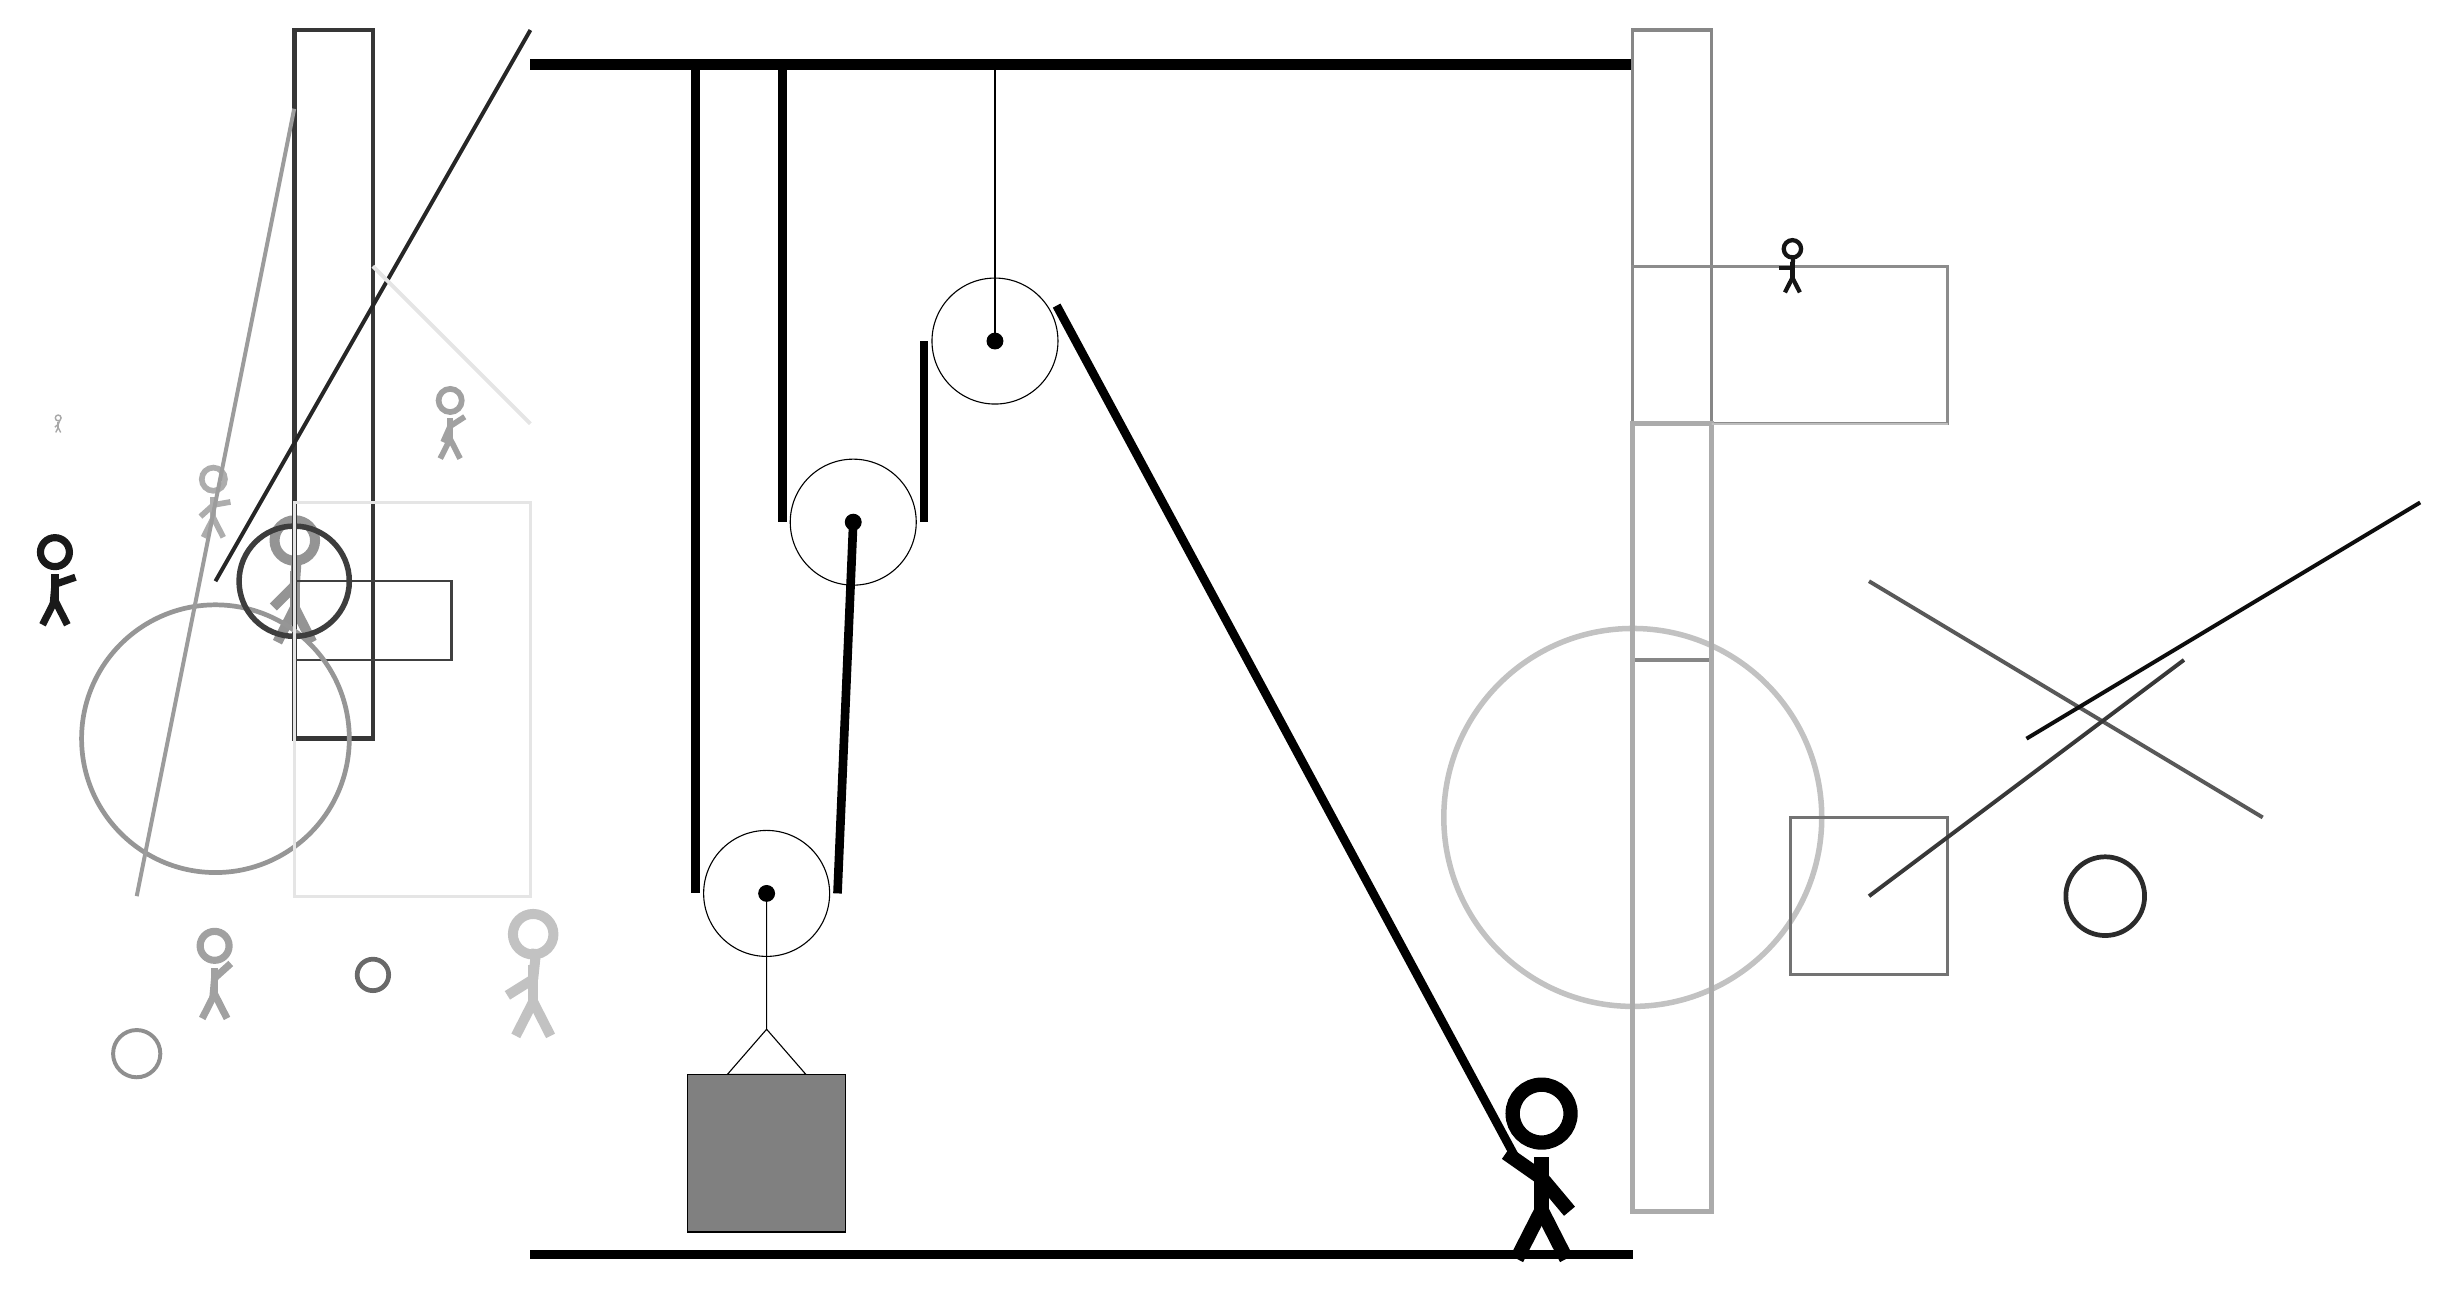
\begin{tikzpicture}
			%%%%% START %%%%%
			
			\draw[fill=black] (-2, 11.5) rectangle (12, 11.625);
			
			\draw (1, 1.035) circle (0.8);
			\draw[fill=black] (1, 1.035) circle (0.1);
			
			\draw (2.1, 5.75) circle (0.8);
			\draw[fill=black] (2.1, 5.75) circle (0.1);
			
			\draw (3.9, 8.05) circle (0.8);
			\draw[fill=black] (3.9, 8.05) circle (0.1);
			\draw[thick] (3.9, 8.05) -- (3.9, 11.5);
			
			\draw[line width=0.4mm, color=black!47] (12, 4) rectangle (13, 12);
			
			\draw [line width=0.7mm, color=black!24](12, 2) circle (2.4);
			\draw [line width=0.5mm, color=black!44](-7, -1) circle (0.3);
			\draw[line width=0.4mm, color=black!55] (14, 0) rectangle (16, 2);
			\node[line width=0.2mm, color=black!37] at (-3, 7) {\Strichmaxerl[4][66][33]};
			\draw[line width=0.2mm, color=black!33] (13, -1) rectangle (13, 6);
			\node[line width=0.6mm, color=black!42] at (-5, 5) {\Strichmaxerl[7][45][86]};
			
			\draw[line width=0.6mm, color=black!79] (-4, 12) rectangle (-5, 3);
			\draw[line width=0.5mm, color=black!85](-2, 12) -- (-6, 5);
			\draw [line width=0.6mm, color=black!83](18, 1) circle (0.5);
			\node[line width=0.2mm, color=black!34] at (-8, 7) {\Strichmaxerl[1][40][68]};
			
			\node[line width=0.2mm, color=black!90] at (-8, 5) {\Strichmaxerl[5][85][19]};
			\draw[line width=0.3mm, color=black!75] (-3, 5) rectangle (-5, 4);
			\node[line width=0.5mm, color=black!24] at (-2, 0) {\Strichmaxerl[7][32][84]};
			\draw[line width=0.5mm, color=black!10](-4, 9) -- (-2, 7);
			\draw[line width=0.5mm, color=black!65](15, 5) -- (20, 2);
			
			\draw[line width=0.5mm, color=black!78](15, 1) -- (19, 4);
			\draw[line width=0.5mm, color=black!95](17, 3) -- (22, 6);
			\draw [line width=0.6mm, color=black!59](-4, 0) circle (0.2);
			\draw [line width=0.6mm, color=black!41](-6, 3) circle (1.7);
			\draw[line width=0.4mm, color=black!45] (12, 9) rectangle (16, 7);
			
			\draw[line width=0.6mm, color=black!33] (12, -3) rectangle (13, 7);
			\node[line width=0.2mm, color=black!92] at (14, 9) {\Strichmaxerl[3][0][86]};
			\node[line width=0.5mm, color=black!32] at (-6, 6) {\Strichmaxerl[4][42][10]};
			\draw [line width=0.7mm, color=black!76](-5, 5) circle (0.7);
			
			\node[line width=0.2mm, color=black!37] at (-6, 0) {\Strichmaxerl[5][85][42]};
			\draw[line width=0.5mm, color=black!39](-7, 1) -- (-5, 11);
			\draw[line width=0.4mm, color=black!10] (-2, 6) rectangle (-5, 1);
			\draw[line width=0.2mm, color=black!26] (13, 7) rectangle (16, 7);
			
			\draw (1, 1.035) -- (1, -0.69) -- (0.5, -1.265) -- (1.5, -1.265) -- (1, -0.69);
			\draw[fill=black!50] (0, -1.265) rectangle (2, -3.265);
			
			\draw[line width=1.1mm] (0.1, 11.5) -- (0.1, 1.035);
			\centerarc[line width=1.1mm](1, 1.035)(180:360:0.9);
			\draw[line width=1.1mm](1.9, 1.035) -- (2.1, 5.75);
			\draw[line width=1.1mm] (1.2, 11.5) -- (1.2, 5.75);
			\centerarc[line width=1.1mm](2.1, 5.75)(180:360:0.9);
			\draw[line width=1.1mm](3.0, 5.75) -- (3.0, 8.05);
			\centerarc[line width=1.1mm](3.9, 8.05)(30:180:0.9);
			\draw[line width=1.1mm] (4.683, 8.5) -- (10.5, -2.3);
			
			\node at (10.8, -2.5) {\Strichmaxerl[10][-35][-50]};
			
			\draw[fill=black] (-2, -3.5) rectangle (12, -3.6);
			
			%%%%% END %%%%%
		\end{tikzpicture}
	\end{figure}	
\end{document}